With the witnesses agreeing on a location, short-range communication, and internal clock synchronization, the infrastructure is ready to generate a verifiable \pol{} certificate. This section will provide a description of the certificate generation process, its requirements, and a possible verification procedure that is derived from the protocol's design. 

Building upon the steps achieved in the previous sections, it is assumed that a zone has been established, and that the zone members are able to achieve time-conscious consensus. Concretely, we assume that both the prover and the witnesses restrict their communications to the zone's physical boundaries, dictated by the coverage of their short-ranged communication means, and we also assume that the zone members are able to achieve zone-relative time synchronization, and so, pace the events of the protocol's execution at the same rate. The next step is to establish the proof generation process, which is based on the zone's relative space and time. The main goal is to assert that the prover is at a specific location, at a specific time, relative to the witnesses. This means, in practical terms, that the prover is able to communicate, via the same short-ranged communication means, with all the witnesses, and is able to demonstrate that it is, as well, synchronized with their internal clocks. However, before asserting such propositions, we also assume that every entity $i$ has a unique key pair, composed of a public key $K^{pu}_i$ and a private key $K^{pr}_i$. The public key represents the identity of an entity, and is used to verify the signature of the messages produced. The private key, on the other hand, is used to sign the messages. The public key of a zone member is known to all the other members, meanwhile, the private keys shall be kept secret. 

Given that the witnesses $w \in W$ are pacing the zone events, i.e., generating new blocks, in average, at every $T$ units of time, and the last block was generated at the zone-relative time $t_x$, with a block hash $h_x$, the proof generation process is as follows:

\begin{enumerate}
    \item The prover $\rho$ synchronizes itself at the zone-relative time $t_x$ and learns the hash  $h_x$ of the last block $B_{x}$.
    \item The prover $\rho$ assembles a transaction $\text{Tx}_\rho$ containing the input $h_x$.
    \item The prover $\rho$ signs the transaction $\text{Tx}_\rho$ with its private key $K^{pr}_\rho$.
    \item The prover $\rho$ broadcasts the transaction $\text{Tx}_\rho$ to the witnesses $w \in W$.
    \item The witnesses $w \in W$ verify the transaction $\text{Tx}_\rho$.
    \item The witnesses $w \in W$ assemble a block $B_{x+1}$ with hash $h_{x+1}$, at time $t_{x+1}$, containing the transaction $\text{Tx}_\rho$.
    \item The witnesses $w \in W$ sign the new block $B_{x+1}$ with their private key $K^{pr}_w$.
    \item The witnesses $w \in W$ broadcast the block $B_{x+1}$ to the entire network.
    \item The prover $\rho$ verifies the hash $h_{x+1}$, the parent hash $h_{x}$, and the signatures of the block $B_{x+1}$, and the inclusion of its transaction $\text{Tx}_\rho$, with the matching input $h_{x}$.
    \item The prover $\rho$, finally, assembles the \pol{} certificate, containing the signed block $B_{x+1}$, by the witnesses $w \in W$, and the signed transaction $\text{Tx}_\rho$, by the prover $\rho$ itself.
\end{enumerate}

Having obtained a valid \pol{} certificate, as the prover $\rho$ was spatially synchronized with the witnesses $w \in W$ around the zone-relative time $t_{x+1}$, the next step would be to submit the certificate to a verification process. Without any verifier-specific information, the verification process would be identical to step 9 of the above procedure. Assuming that the verifier knows the identities of all the entities involved in the proof generation process, the verification process would go around verifying the signatures of both the block $B_{x+1}$ and the transaction $\text{Tx}_\rho$, by the witnesses and the prover, respectively, and verifying, as well, that the transaction input matches the parent hash $h_{x}$ of the block. This last verification step ensures that the prover was spatially synchronized with the witnesses around the zone-relative time $t_{x+1}$. A more well-founded analysis of the robustness, security, privacy, and, eventually, the correctness of this \pol{} protocol, inspired by the works presented in Chapter~\ref{sec:related-work}, is left for future work. This would, as well, include a more detailed analysis of the security against the most common attacks and collusion scenarios, like proxy attacks or witness collusions. Bridging with the examples presented in Figure~\ref{fig:proof-of-location-example-scenarios}, in the first use case, the prover is represented by the reporter, and the witnesses are the bystanders that are passing by the accident site. The goal of the reporter is to prove that he was physically present at the location of the accident, factually covering the event. The proof, possibly containing a piece of media content, is attested by the onlookers and verified by a journalist when producing a news piece. In the second case, the ISP assumes the prover role and tries to gather a proof of the service provision within the customers' neighbourhood. Ultimately, the proof can be verified by regulators that are responsible for the enforcement of service level agreements.

\newpage  

\begin{figure}[h!]
    \begin{center}
    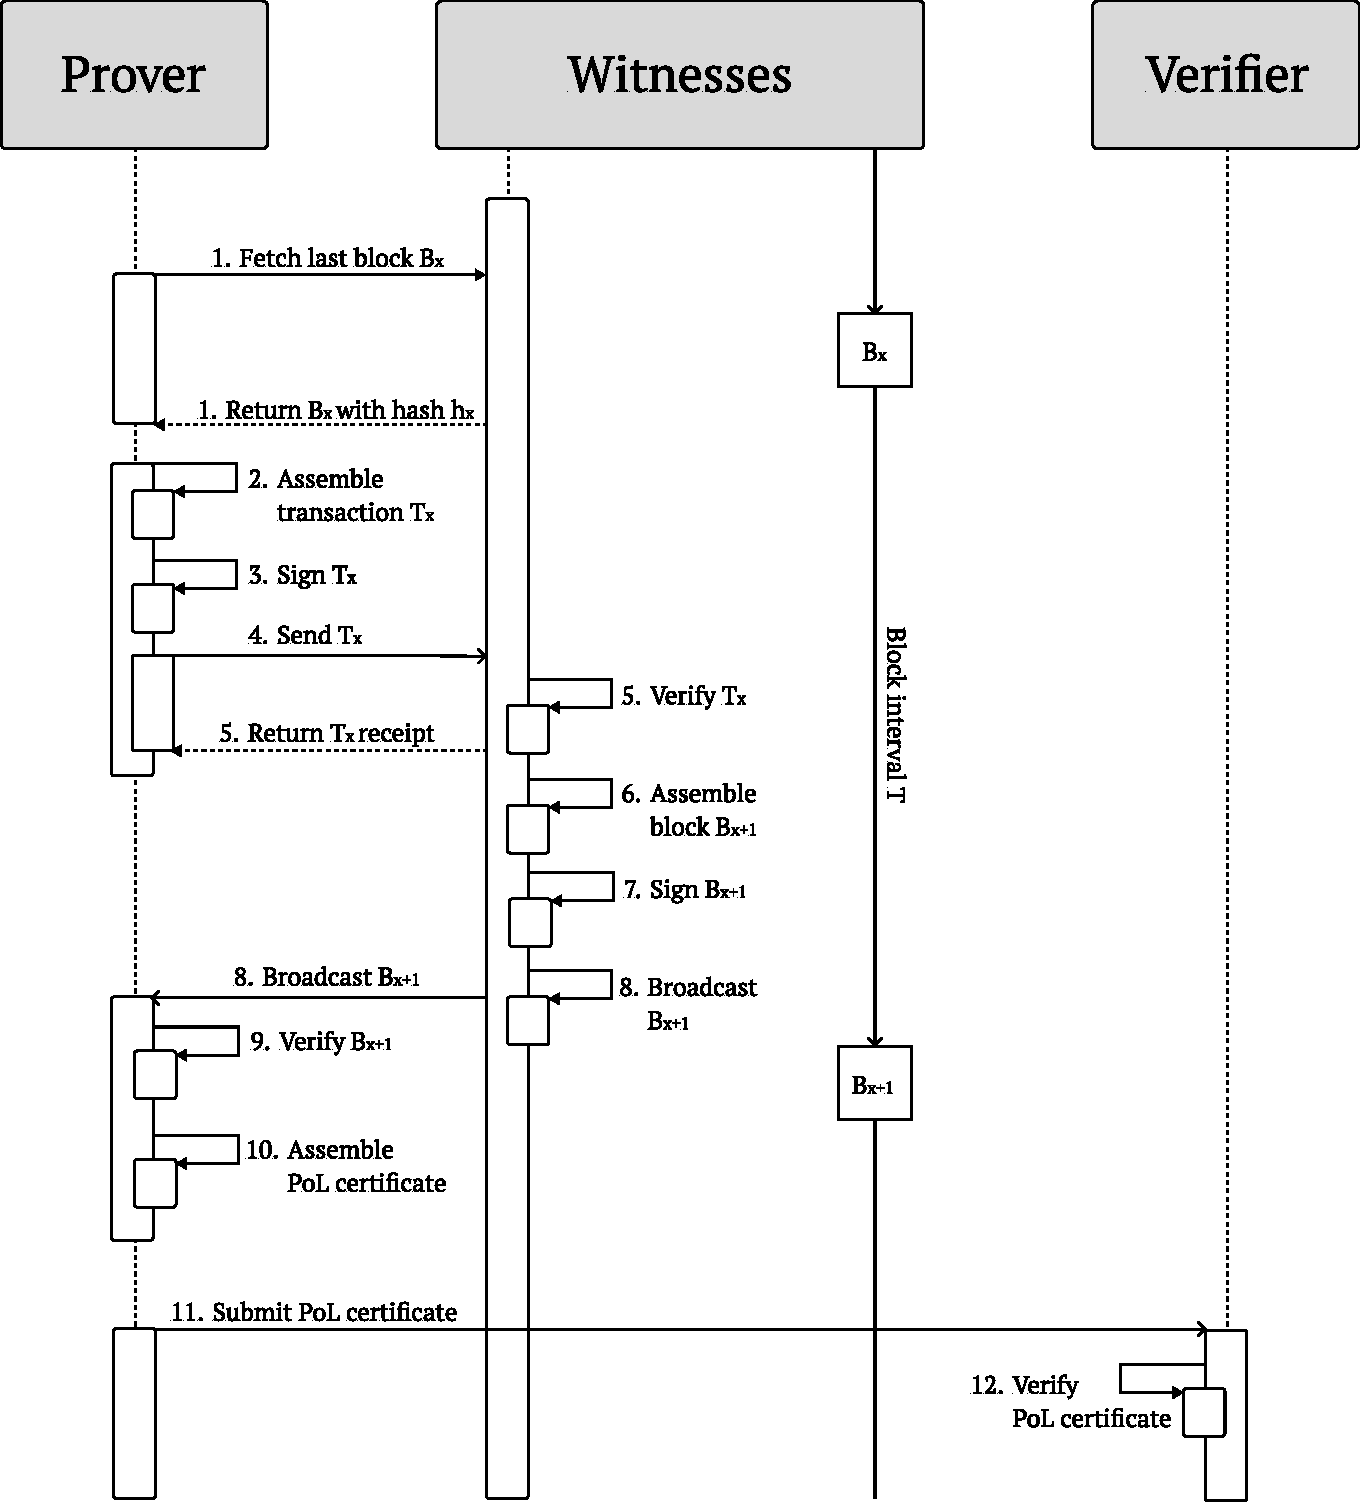
\includegraphics[width=\textwidth]{overview-pol-rel-seq.pdf}
    \caption{Sequence diagram overview of the proof generation process.}
    \vspace{-0.5cm}
    \label{fig:proof-of-location-overview-relative-pol-seq}
    \end{center}
\end{figure}

Up to this point, the protocol has been described in a relative manner, i.e., the prover is able to prove its location relative to the witnesses. The underlying mesh network enabled the short-ranged communication, while a permissionless consensus mechanism allowed for the time synchronization and generation of a verifiable certificate. The next section will provide a rough outline of how this protocol can be extended to achieve Absolute \pol{}, involving the introduction of verified space and time references.